\documentclass[%twocolumn,
amssymb,prb,aps,superscriptaddress]{revtex4}

\usepackage{graphicx}
\usepackage[utf8]{inputenc}
\usepackage{float}

\usepackage{amsmath}
\usepackage{amssymb}
\usepackage{amsthm}
\usepackage{amsfonts}
\usepackage{braket}


\begin{document}

\begin{abstract}
    Hola Abstract, este es un pequeño resumen del documento presentado
\end{abstract}

\title{Resonancia Paramagnetica Spin Electrón}
\author{Majo}

\affiliation{Colegio de Ciencias e Ingeniería, USFQ, Quito, Ecuador} 

\author{Martin}

\affiliation{Colegio de Ciencias e Ingeniería, USFQ, Quito, Ecuador}

\date{\today}

\maketitle

\section[Intro]{Introducción}
\label{sec:intro}

Lo que es, de donde sale, quien lo descubrio, lo que dice en wikipedia y que vamos a decir en paper

\section[]{Cuántica del Sistema}
\label{sec:cuantica}

\subsection{Prototipo Hamiltoniano}

El prototipo basico de RPE es una interaccion entre 2 particulas de Spin $1/2$, el proton del nucleo con spin $\vec{I}$ y el del $e^-$ $\vec{S}$. El hamiltoniano del sistema electron nucleo puede escribirse con terminos de la interacción entre los 2 spines $ \vec{I} \cdot \vec{S} $ y los terminos de Zeeman $g \beta \vec{H} \cdot \vec{J}$, si asumimos que el $\vec{H}$ esta en $z$ tenemos

\begin{equation}
    \label{eq:hamiltonianoDelSistema}
    \mathcal{\hat{H}} = H (g_e \beta \hat{S_z} - g_N \beta_N \hat{I_z}) + T \vec{S} \cdot \vec{I} 
\end{equation}

\subsection{Prototipo Solución}

Para la solución vamos a usar la base de spin nucleo y electron acoplada $\hat{\vec{J}} = \hat{\vec{S}} + \hat{\vec{L}}$. En el orden $\ket{0,0}$, $\ket{1,-1}$, $\ket{1,0}$, $\ket{1,+1}$. En esta base y usando el hecho que $ 2 \hat{\vec{I}} \cdot \hat{\vec{S}} = \hat{J^2} - \hat{S^2} - \hat{I^2} $ tenemos la matriz de $\mathcal{\hat{H}}$

$$
\hat{\mathcal{H}} =     
\begin{pmatrix}

    -\frac{3}{2} T \hbar^2 & 0 & - \frac{H \hbar}{2} (g_e \beta_e + g_N \beta_N) & 0 \\

    0 & -\frac{H \hbar}{2} (g_e \beta_e - g_N \beta_N) + \frac{T \hbar^2}{4} & 0 & 0 \\

    - \frac{H \hbar}{2} (g_e \beta_e + g_N \beta_N) & 0 & \frac{T \hbar^2}{4} & 0 \\

    0 & 0 & 0 & \frac{H \hbar}{2} (g_e \beta_e - g_N \beta_N) + \frac{T \hbar^2}{4} \\

\end{pmatrix}
$$

Los valores propios del hamiltoniano o las energias posibles del sistema son

%\begin{equation}
    \begin{align*}
        E_1 = \frac{\hbar}{4}(T \hbar - 2 H (g_e \beta_e - g_N \beta_N)) \\
        E_2 = \frac{\hbar}{4}(T \hbar + 2 H (g_e \beta_e - g_N \beta_N)) \\
        E_3 = \frac{\hbar}{8}\left(-5 T \hbar - \sqrt{\frac{8^2 H^2}{2^2} (g_e \beta_e + g_N \beta_N)^2 + 7^2 T^2 \hbar^2}\right) \\
        E_4 = \frac{\hbar}{8}\left(-5 T \hbar + \sqrt{\frac{8^2 H^2}{2^2} (g_e \beta_e + g_N \beta_N)^2 + 7^2 T^2 \hbar^2} \right) \\
    \end{align*}
%\end{equation}

usando la aproximacion comun en RPE de $$ g_a \beta_a \hbar >> T  $$
tenemos

%\begin{equation}
    \begin{align*}
        E_1 = \frac{\hbar}{4}(T \hbar - 2 H (g_e \beta_e - g_N \beta_N)) \\
        E_2 = \frac{\hbar}{4}(T \hbar + 2 H (g_e \beta_e - g_N \beta_N)) \\
        E_3 = \frac{\hbar}{8}\left(-5 T \hbar - 4 H (g_e \beta_e + g_N \beta_N)\right) \\
        E_4 = \frac{\hbar}{8}\left(-5 T \hbar + {4 H} (g_e \beta_e + g_N \beta_N)\right) \\
    \end{align*}
%\end{equation}

    \begin{figure}[H]
        \centering
        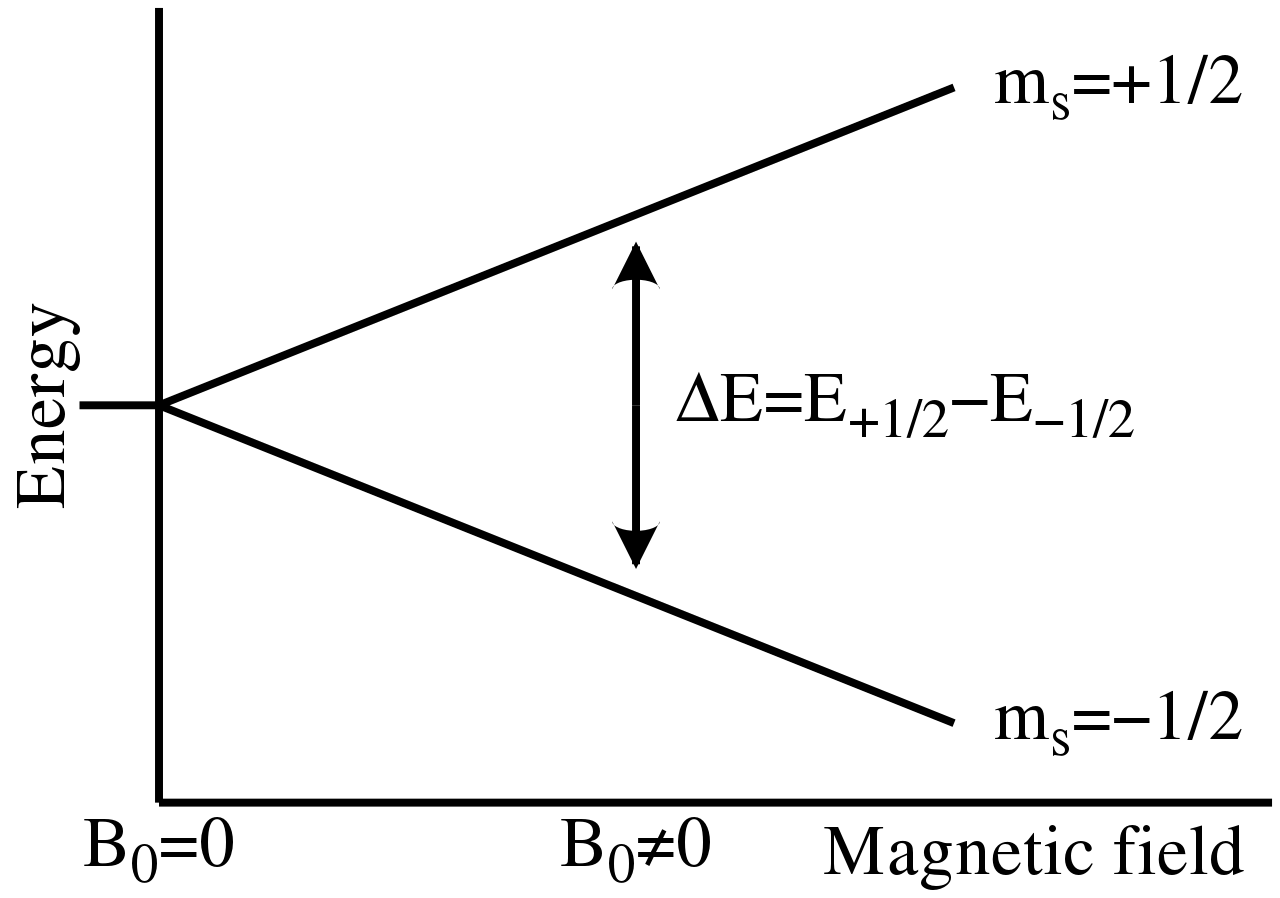
\includegraphics[width=6.0cm]{images/EPR_splitting}
        \caption{Diagrama de diferencia de Energia}
        \label{fig:diagramaDiferenciaDeEnergia} \label{sec:momentosAngulares}

        \subsection{interacción Spin Campo}
    \end{figure}

\section{Aplicaciones}
\label{sec:aplicacion1}

\subsection{Espectroscopia}
\label{sec:aplicacion2}

\subsection{Metales}

\subsection{Datacion}

\end{document}